% XeLaTeX can use any Mac OS X font. See the setromanfont command below.
% Input to XeLaTeX is full Unicode, so Unicode characters can be typed directly into the source.

% The next lines tell TeXShop to typeset with xelatex, and to open and save the source with Unicode encoding.

%!TEX TS-program = xelatex
%!TEX encoding = UTF-8 Unicode

\documentclass[12pt]{article}
\usepackage{geometry}                % See geometry.pdf to learn the layout options. There are lots.
\geometry{letterpaper}                   % ... or a4paper or a5paper or ... 
%\geometry{landscape}                % Activate for for rotated page geometry
%\usepackage[parfill]{parskip}    % Activate to begin paragraphs with an empty line rather than an indent
\usepackage{graphicx}
\usepackage{caption}
\usepackage{subcaption}
\usepackage{amssymb}

% Will Robertson's fontspec.sty can be used to simplify font choices.
% To experiment, open /Applications/Font Book to examine the fonts provided on Mac OS X,
% and change "Hoefler Text" to any of these choices.

\usepackage{fontspec,xltxtra,xunicode}
\defaultfontfeatures{Mapping=tex-text}
\setromanfont[Mapping=tex-text]{Hoefler Text}
\setsansfont[Scale=MatchLowercase,Mapping=tex-text]{Arial}
\setmainfont[Scale=.95]{Times}
\setmonofont[Scale=MatchLowercase]{Consolas}

\title{Permutations and FST Lattices}
\author{Josef R. Novak}
\date{}                                           % Activate to display a given date or no date

\begin{document}
\maketitle

\section{The best permutation}
This document provides a minimal, graphical example describing how to compute the most likely permutation of a word list given an input statistical language model, using a cascaded, WFST-based algorithm.  Given a list of $N$ input words, for example,
\begin{verbatim}
       to goes he the park
\end{verbatim}
\noindent we may wish to compute the most likely sequence given some probabilistic model.  A simple but not very efficient method to do this would be to simply iterate through each possible permutation and track the most likely candidate given the reference language model.  This will work, but it will require iterating through $N!$ possible permutations in the worst case.  Instead we would like to find a slightly more efficient approach.

\section{Cascaded Counters}
It is possible to achieve a more efficient result by computing a compact lattice representation of the set of permutations.  We can achieve this by cascading a series of counter-like FSTs, which enforce constraints on the number of times each word is permitted to occur.  The first step is build a ``skeleton'' FSA that enforces no restrictions other than length.  Using the example toy input list, \verb|a b c c|, this first step would result in a skeleton FSA like that depicted in Figure~\ref{fig:cmp0}.
\begin{figure}[th!]
\begin{center}
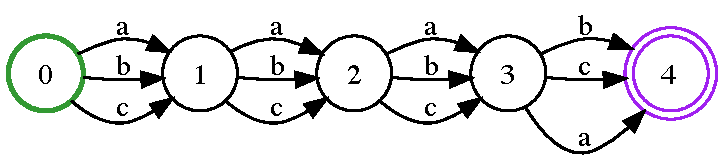
\includegraphics[width=.8\textwidth]{cmp0}
\caption{Skeleton FSA corresponding to the toy input word list ``\texttt{a b c c}''.}
\label{fig:cmp0}
\end{center}
\end{figure}
Next we construct a counter FSA for each word, which reflects the number of times each word is permitted to occur.  The counters for the input example are depicted in Figure~\ref{fig:cmp1}--Figure~\ref{fig:cmp3}.
\begin{figure}
        \centering
        \begin{subfigure}[b]{0.25\textwidth}
                \centering
                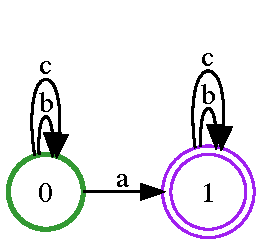
\includegraphics[width=\textwidth]{cmp1}
                \caption{FSA for word ``\texttt{a}'''.}
                \label{fig:cmp1}
        \end{subfigure}%
        ~ %add desired spacing between images, e. g. ~, \quad, \qquad etc. 
          %(or a blank line to force the subfigure onto a new line)
        \begin{subfigure}[b]{0.25\textwidth}
                \centering
                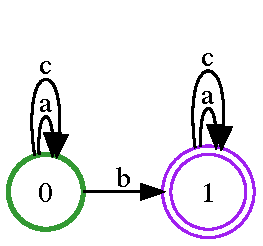
\includegraphics[width=\textwidth]{cmp2}
                \caption{FSA for word ``\texttt{b}'''.}
                \label{fig:cmp2}
        \end{subfigure}
        ~ %add desired spacing between images, e. g. ~, \quad, \qquad etc. 
          %(or a blank line to force the subfigure onto a new line)
        \begin{subfigure}[b]{0.4\textwidth}
                \centering
                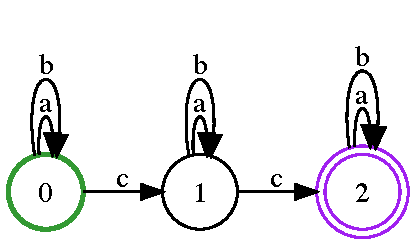
\includegraphics[width=\textwidth]{cmp3}
                \caption{FSA for word ``\texttt{c}'''.}
                \label{fig:cmp3}
        \end{subfigure}
        \caption{Enforcement FSAs for component words.}\label{fig:enforcers}
\end{figure}
Finally the lattice of possible permutations can be constructed by simply cascading the the components together via weighted composition, as described in Equation~\ref{eq:cascade},
\begin{equation}\label{eq:cascade}
 C = (c\circ (b\circ (a\circ S)))
\end{equation}
where $S$ represents the skeleton FSA and $a$, $b$, and $c$ represent the component enforcement FSAs.  This will produce the compact FSA lattice depicted in Figure~\ref{fig:cascade}.
\begin{figure}[h!]
\begin{center}
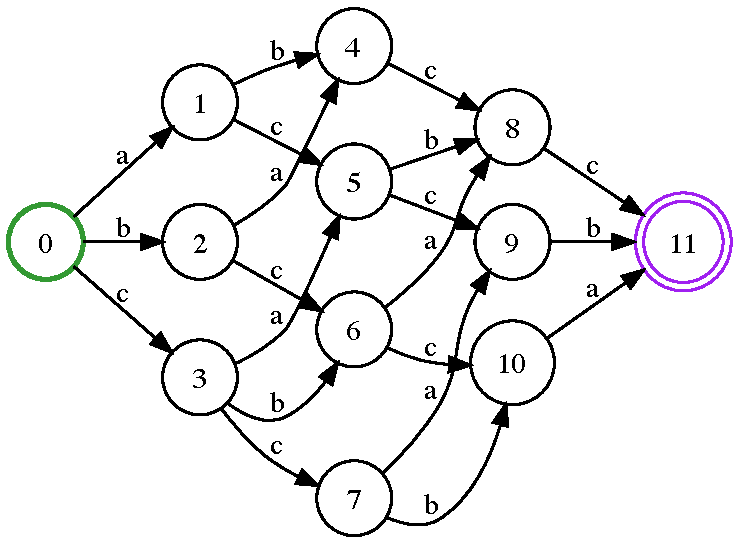
\includegraphics[width=.7\textwidth]{cascade}
\end{center}
\caption{FSA-based permutation lattice resulting from composition of skeleton FSA and component enforcement FSAs.}
\label{fig:cascade}
\end{figure}
\clearpage 
\noindent In the case of the lattice based method each composition operation requires Time: $O(V_{1} V_{2} D_{1}\cdot (log D_{2} + M_{2}))$, Space: $O(V_{1} V_{2} D_{1} M_{2})$ where $V_{i} =$ \# of states visited, $D_{i} =$ maximum out-degree, and $M_{i} =$ maximum multiplicity of the states visited for the $i^{th}$ FST~\cite{openfst}.  The resulting cascade may then be composed with the WFSA-based representation of the LM just one time, and the shortest path algorithm can be utilized to compute the most likely permutation.  The shortest path algorithm then requires just Time: $O(V log V + E)$, Space: $O(V)$.  In general this is significantly more efficient than the brute force method, particularly for longer word lists.

The included evaluation utility, ``\texttt{compute-best-permutation}'' also provides timing information, which can be used to compare the two methods discussed above.
% using the International Panel in System Preferences.
% Unicode must be typeset using a font containing the appropriate characters.
% Remove the comment signs below for examples.

% \newfontfamily{\A}{Geeza Pro}
% \newfontfamily{\H}[Scale=0.9]{Lucida Grande}
% \newfontfamily{\J}[Scale=0.85]{Osaka}

% Here are some multilingual Unicode fonts: this is Arabic text: {\A السلام عليكم}, this is Hebrew: {\H שלום}, 
% and here's some Japanese: {\J 今日は}.
\footnotesize
 \begin{thebibliography}{99}

\bibitem{openfst} Allauzen, C., et al. M.~A. and Bork, P. 1998. Measuring genome evolution. {\em Open{F}st: A General and Efficient Weighted Finite-State Transducer Library}, CIAA 2007, pp. 11--23.

\end{thebibliography}


\end{document}  